\documentclass[11pt]{article}
\usepackage{amssymb}
\usepackage{tikz}
\usepackage{fancyhdr}
\usepackage{extramarks}
\usepackage{pgfplots}
\usetikzlibrary{automata,positioning}
\usetikzlibrary{shapes.geometric, arrows}


\setlength{\topmargin}{-1.5in}
\setlength{\textheight}{9.5in}
\setlength{\oddsidemargin}{.125in}
\setlength{\textwidth}{6.25in}

\tikzstyle{startstop} = [rectangle, rounded corners, minimum width=3cm, minimum height=1cm,text centered, text width=3cm, draw=black, fill=red!30]
\tikzstyle{basicblock} = [rectangle, minimum width=3cm, minimum height=1cm,text centered, text width=3cm, draw=black, fill=blue!30]

\tikzstyle{io} = [trapezium, trapezium left angle=70, trapezium right angle=110, minimum width=3cm, minimum height=1cm, text centered, text width=2cm,draw=black, fill=blue!30]
\tikzstyle{process} = [rectangle, minimum width=3cm, minimum height=1cm, text centered, text width=2cm,draw=black, fill=orange!30]
\tikzstyle{decision} = [diamond, minimum width=3cm, minimum height=1cm, text centered, text width=2cm, draw=black, fill=green!30]



\tikzstyle{arrow} = [thick,->,>=stealth]
\begin{document}
	\title{
		\textbf{Car Logic Architecture}
	}
	\date{}
	\maketitle

	\begin{tikzpicture}[node distance=2.5cm]


% Launch script

	\node (launchd) [startstop, xshift=1cm] {Launcd};


% Simulations

	\node (sumo)[basicblock, below of=launchd, xshift=-3cm] {Sumo};

	\node(omnet)[basicblock, below of=launchd, xshift=3cm]{Omnet};


% Car stack

	\node (hardwareSim)[basicblock, below of=sumo] {Hardware Simulation};

	\node (agents) [basicblock, below of=hardwareSim] {Agents};


% Network stack

	\node(omnetPY)[basicblock, below of=omnet]{Omnet.py interface};

	\node(meshNet)[io, below of=omnetPY]{Mesh Network};


% API

	\node (carLogicAPI)[io, below of=agents, xshift=3cm]{Car Logic API};


% Controller

	\node(loopStatement)[startstop, left of=agents, xshift=-2cm]{Continously loop and run each agent\, step simulation};






% Launchd statement arrows
	\draw [arrow] (launchd.170) -| (loopStatement);

	\draw [arrow] (launchd) -| node[ anchor=east, yshift=-1cm]{Open Sumo} (sumo);
	\draw [arrow] (launchd) -| node [anchor=west, yshift=-1cm]{Open Omnet}(omnet);



% Omnet - Sumo connection
	\draw [arrow] (omnet.170)--(sumo.10);
	\draw [arrow] (sumo.350)--(omnet.190);


% Network Stack
	\draw [arrow] (omnet.250) -- (omnetPY.110);
	\draw [arrow] (omnetPY.70) -- (omnet.290);

	\draw [arrow] (omnetPY.250) -- (meshNet.110);
	\draw [arrow] (meshNet.70) -- (omnetPY.290);


% Hardware Stack
	\draw [arrow] (sumo.250) -- (hardwareSim.110);
	\draw [arrow] (hardwareSim.70) -- (sumo.290);

	\draw [arrow] (hardwareSim.250) -- (agents.110);
	\draw [arrow] (agents.70) -- (hardwareSim.290);


% Car logic API connects
	\draw [arrow] (meshNet.250) |- (carLogicAPI.10);
	\draw [arrow] (carLogicAPI.350) -| (meshNet.290);

	\draw [arrow] (agents.290) |- (carLogicAPI.170);
	\draw [arrow] (carLogicAPI.190) -| (agents.250);


% Loop of all agents, sumulation control
	\draw [arrow] (agents.170) -- (loopStatement.10);
	\draw [arrow] (loopStatement.350) -- (agents.190);


	\end{tikzpicture}

	\begin{enumerate}
		\item Launchd: Describe here
		\item Sumo: Describe here
		\item Omnet: Describe here
		\item ?: Describe here
		\item Omnet.py: Describe here


	\end{enumerate}
\end{document}
